\documentclass[11pt,letter]{article}

\usepackage[margin=1in]{geometry}
\usepackage{graphicx}
\usepackage{amssymb}
\usepackage{amsmath}
\usepackage{multirow}
\usepackage{epstopdf}
\usepackage{setspace}
\usepackage{currfile}
\usepackage[abbr]{harvard}
\usepackage[pagewise]{lineno}
\usepackage{xcolor}
\usepackage{framed}
\definecolor{shadecolor}{rgb}{0.9,0.9,0.9}
\usepackage{tcolorbox}
\usepackage{gensymb}
\usepackage{pdfpages}
\usepackage{graphics}

\DeclareMathOperator{\Be}{Be}
\DeclareMathOperator{\tr}{tr}
\DeclareMathOperator{\sd}{sd}
\DeclareMathOperator{\var}{Var}
\DeclareMathOperator{\cov}{Cov}
\DeclareMathOperator{\diag}{diag}

\usepackage{hyperref}
\hypersetup{
    colorlinks,
    citecolor=black,
    filecolor=black,
    linkcolor=black,
    urlcolor=black
}
\usepackage{authblk}

%\setpagewiselinenumbers
%\modulolinenumbers[5]
%\linenumbers
%\doublespace
%\setstretch{1.5}

\title{Supplement to ``Testing axioms of stochastic discrete choice using population choice probabilities''}
\author[1]{William J. McCausland\thanks{william.j.mccausland@umontreal.ca, File: \texttt{\currfilename}, Very preliminary.}}
\author[2]{A.A.J. Marley \thanks{ajmarley@uvic.ca}}
\author[3]{Clintin Davis-Stober}
\affil[1]{Universit\'e de Montr\'eal}
\affil[2]{University of Victoria}
\affil[3]{University of Missouri}

\renewcommand\Authands{ and }

\begin{document}

\maketitle

\begin{abstract}
	This is a supplement.
\end{abstract}

\section{Domains}\label{s:domains}

\pagebreak

\subsection*{Male stars}
%%%%%%%%%%%%%%%%%%%%%%%%

% Male stars

The source for this domain is the website \texttt{ranker.com}, accessed June 4, 2017.
The list is ``The best actors working today''.
The choices are the top five actors in that list, in order.

\begin{tcolorbox}
Which movie star would you choose to have lunch with?

\begin{itemize}
	\setlength\itemsep{-5pt}
	\item Tom Hanks
	\item Kevin Spacey
	\item Morgan Freeman
	\item Leonardo DiCaprio
	\item Christian Bale
\end{itemize}
\end{tcolorbox}

\subsubsection*{Random screenshot}

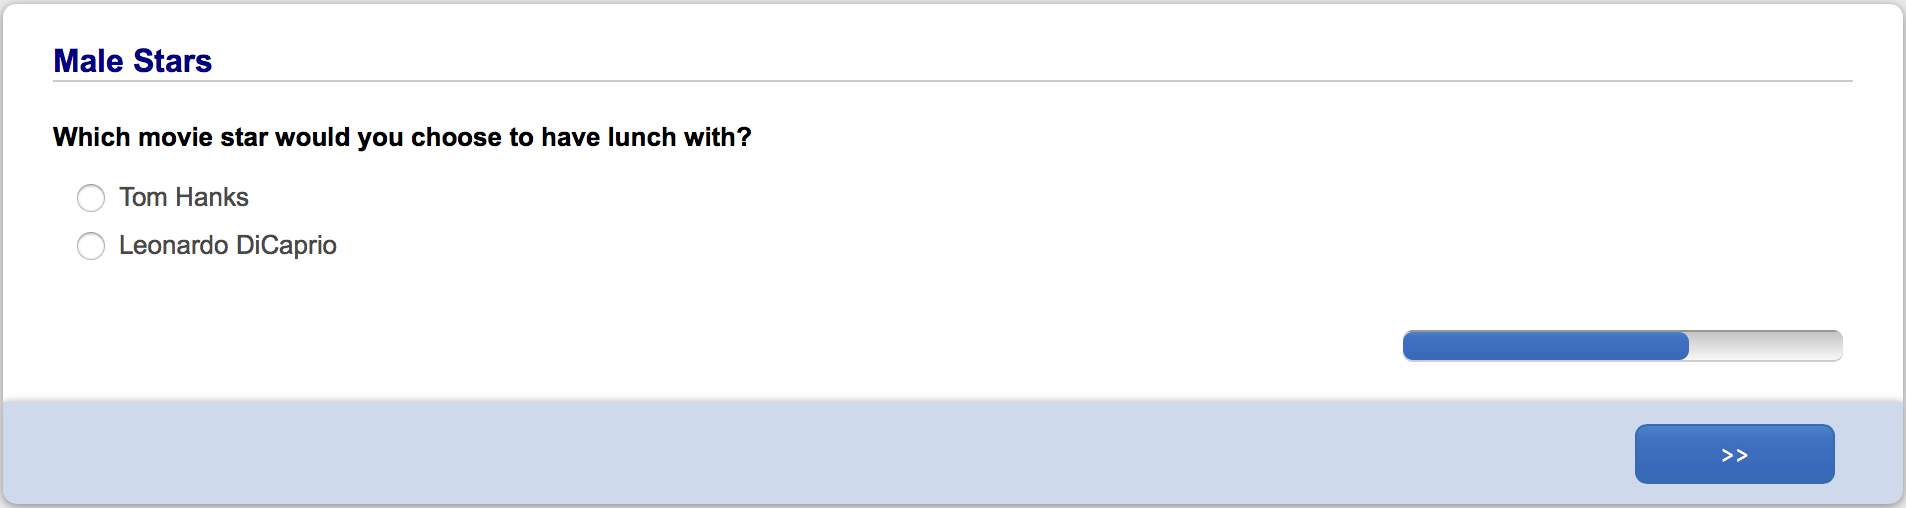
\includegraphics[width=15cm]{Population_study_design/screenshot_Male_Stars.png}

\subsubsection*{Observed binary and ternary choices}

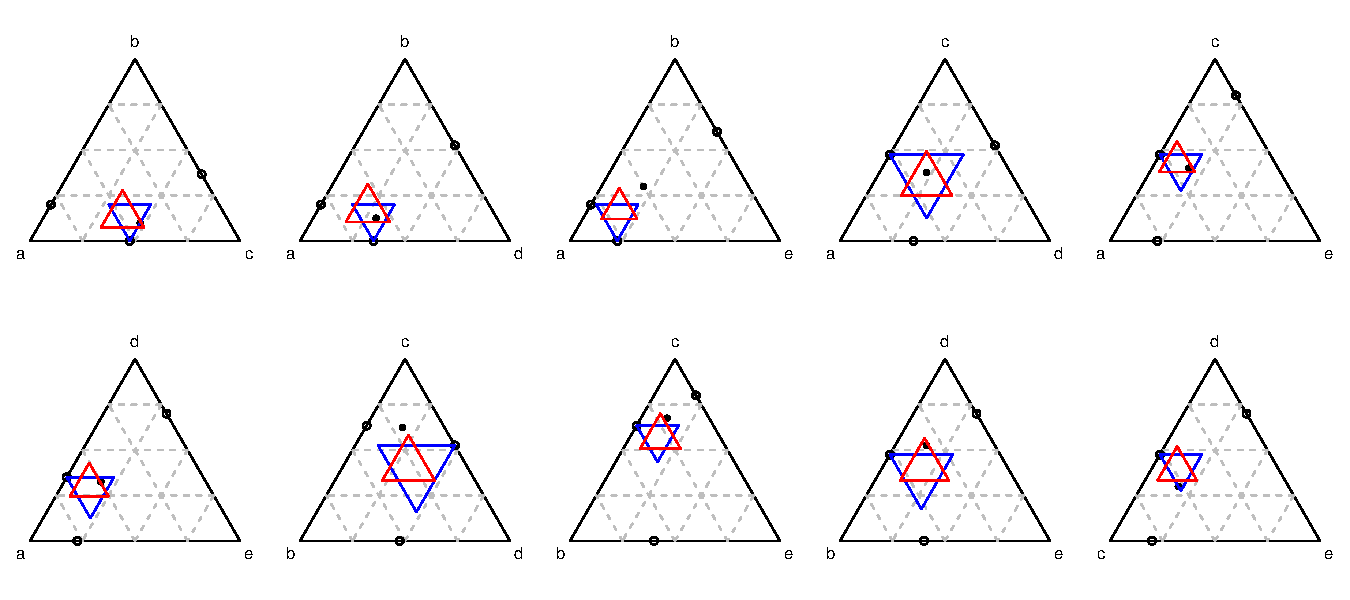
\includegraphics[width=15cm]{./Population_study_data/Simplexes/Male_stars.pdf}

\pagebreak

\subsection*{Female stars}
%%%%%%%%%%%%%%%%%%%%%%%%%

% Female stars

The source for this domain is the website \texttt{ranker.com}, accessed June 4, 2017.
The list is ``The best American actresses working today''.
These are the top five actors in that list, in order.
Jodie Foster's name was misspelled in the experiment, as two participants noted in the comments.

\begin{tcolorbox}
Which movie star would you choose to have lunch with?

\begin{itemize}
	\setlength\itemsep{-5pt}
	\item Meryl Streep
	\item Jody Foster
	\item Kathy Bates
	\item Amy Adams
	\item Julianne Moore
\end{itemize}
\end{tcolorbox}


\subsubsection*{Random screenshot}

\includegraphics[width=15cm]{Population_study_design/screenshot_female_Stars.png}

\subsubsection*{Observed binary and ternary choices}

\includegraphics[width=15cm]{./Population_study_data/Simplexes/female_stars.pdf}

\pagebreak

\subsection*{Films}
%%%%%%%%%%%%%%%%%%

% Films

The source for this domain is the IMDb list ``Most Popular Feature Films Released 1990 to
1999''.
The decade was chosen so that the films would not be easily recognizable by most respondents.

\begin{tcolorbox}
Judging from the following descriptions of films, which one of the films would you choose to see?

\begin{itemize}
	\setlength\itemsep{-15pt}
	\item Two imprisoned men bond over a number of years, finding solace and
eventual redemption through acts of common decency. \\
	\item Mathilda, a 12-year-old girl, is reluctantly taken in by L\'eon, a
professional assassin, after her family is murdered. L\'eon and Mathilda
form an unusual relationship, as she becomes his prot\'eg\'e and learns the
assassin's trade. \\
	\item The lives of two mob hit men, a boxer, a gangster's wife, and a pair
of diner bandits intertwine in four tales of violence and redemption. \\
	\item A sexually frustrated suburban father has a mid-life crisis after
becoming infatuated with his daughter's best friend. \\
	\item Identical twins, separated at birth and each raised by one of their
biological parents, discover each other for the first time at summer camp
and make a plan to bring their wayward parents back together.
\end{itemize}
\end{tcolorbox}


\subsubsection*{Random screenshot}

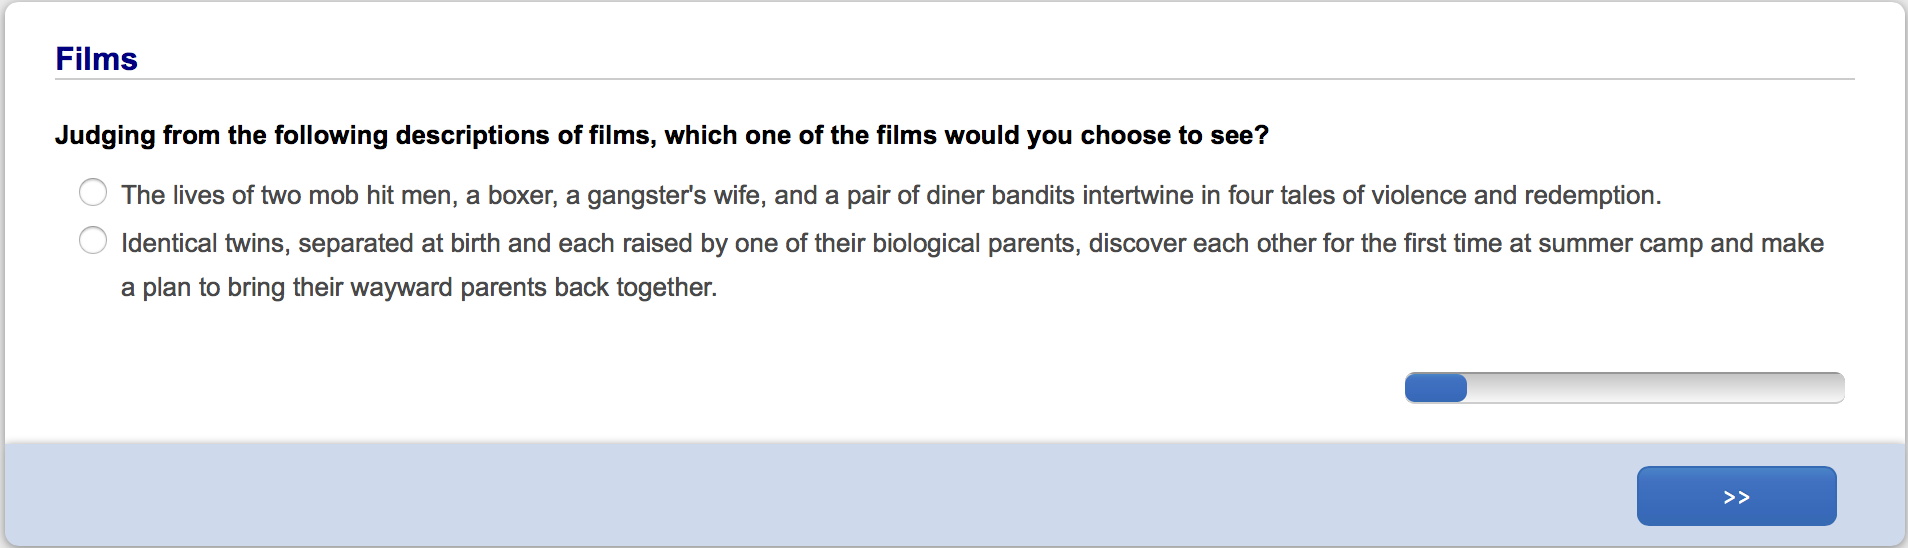
\includegraphics[width=15cm]{Population_study_design/screenshot_films.png}

\subsubsection*{Observed binary and ternary choices}

\includegraphics[width=15cm]{./Population_study_data/Simplexes/films.pdf}

\pagebreak

\subsection*{Star pairs}
%%%%%%%%%%%%%%%%%%%%%%%

% Star pairs

Here, choice objects are pairs of movie stars from a set of four movie stars: Tom Hanks, Scarlett Johansson, Brad Pitt and Angelina Jolie.
The only missing pair is Brad Pitt and Angelina Jolie.
One possible measure of similarity is the number of actors in common between two pairs, with values 0 and 1.
There are nine doubleton choice sets (i.e. pairs of actor pairs) with one star in common and one ($\{c,d\}$) without any stars in common.
Thus there are three triples ($\{a,c,d\}$, $\{b,c,d\}$, $\{c,d,e\}$) where one might expect a similarity effect.

In this example, respondents' preferences may depend not only on their liking of particular actors but also on complementaries between actors.
{}
\begin{tcolorbox}
Knowing only who is starring, which one of these new films would you choose to see?

\begin{itemize}
	\setlength\itemsep{-5pt}
	\item Tom Hanks and Scarlett Johansson
	\item Scarlett Johansson and Brad Pitt
	\item Tom Hanks and Brad Pitt
	\item Scarlett Johansson and Angelina Jolie
	\item Tom Hanks and Angelina Jolie
\end{itemize}
\end{tcolorbox}


\subsubsection*{Random screenshot}

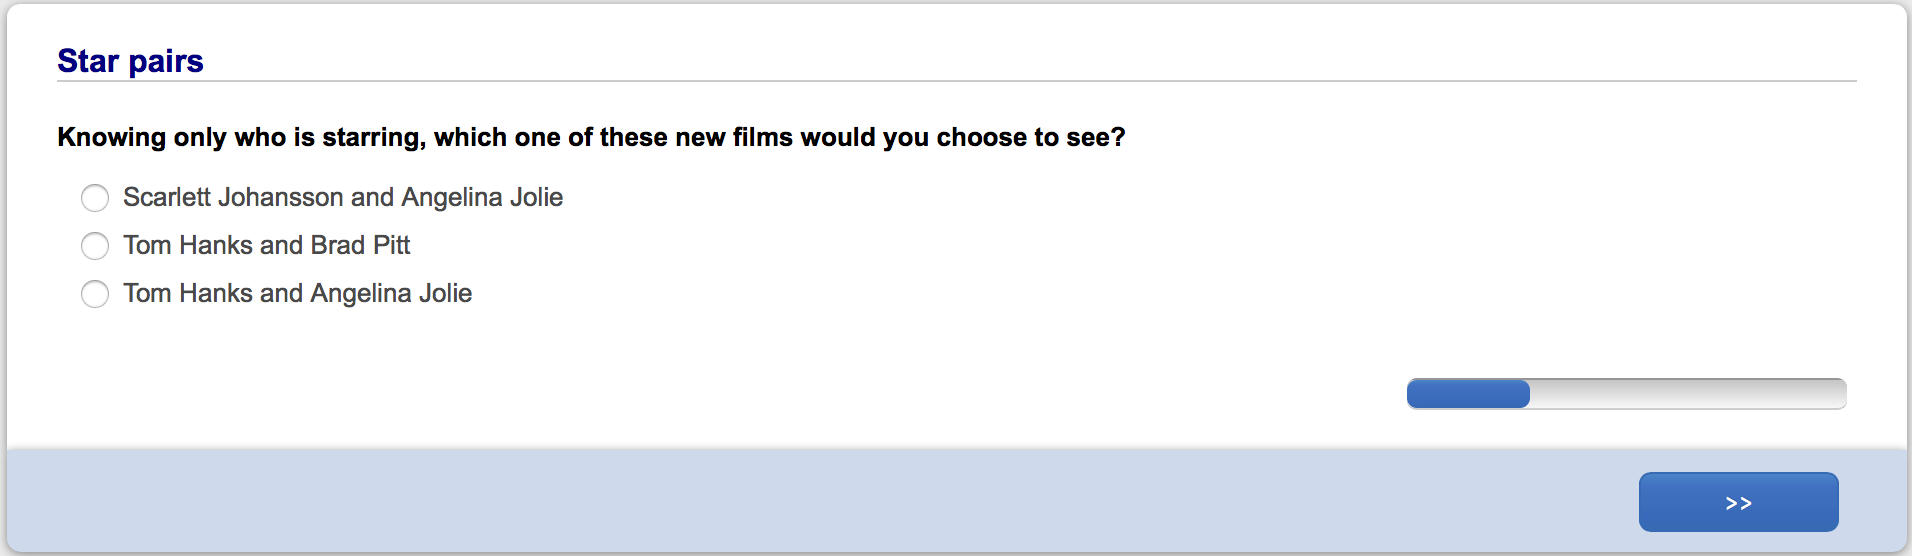
\includegraphics[width=15cm]{Population_study_design/screenshot_star_pairs.png}

\subsubsection*{Observed binary and ternary choices}

\includegraphics[width=15cm]{./Population_study_data/Simplexes/star_pairs.pdf}

\pagebreak

\subsection*{Pizzas}
%%%%%%%%%%%%%%%%%%%

% Pizzas

The source for this domain is a Montreal pizza restaurant.
All these pizzas are either 12 or 13 dollars.

\begin{tcolorbox}
Which one of the following pizzas would you choose?

\begin{itemize}
	\setlength\itemsep{-5pt}
	\item Mozzarella, tomato sauce, basil
	\item Pepperoni, mushrooms, green pepper, mozzarella, tomato sauce
	\item Red onion, tomato sauce, feta, mozzarella, olive oil, Greek spices,
tomato sauce
	\item Bacon, white onion, mozzarella, parmesan, fresh cream, tomato sauce,
ground pepper
	\item Mushrooms, green pepper, mozzarella, tomato sauce
\end{itemize}
\end{tcolorbox}


\subsubsection*{Random screenshot}

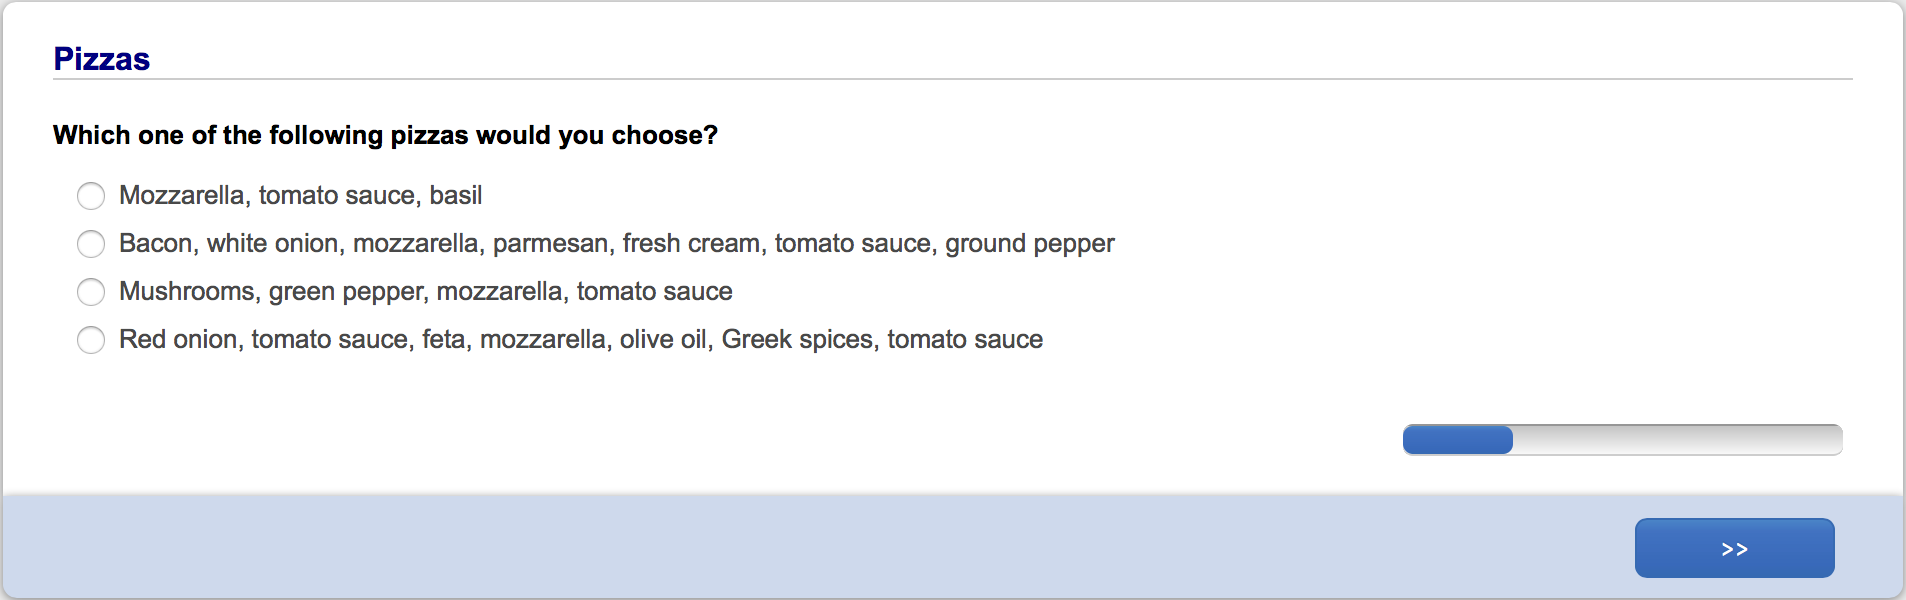
\includegraphics[width=15cm]{Population_study_design/screenshot_pizzas.png}

\subsubsection*{Observed binary and ternary choices}

\includegraphics[width=15cm]{./Population_study_data/Simplexes/pizzas.pdf}

\pagebreak

\subsection*{Juices}
%%%%%%%%%%%%%%%%%%%

% Juices

\begin{tcolorbox}
Which one of the following fresh juices would you choose?

\begin{itemize}
	\setlength\itemsep{-5pt}
	\item Mango
	\item Orange
	\item Apple
	\item Grapefruit
	\item Pineapple
\end{itemize}
\end{tcolorbox}


\subsubsection*{Random screenshot}

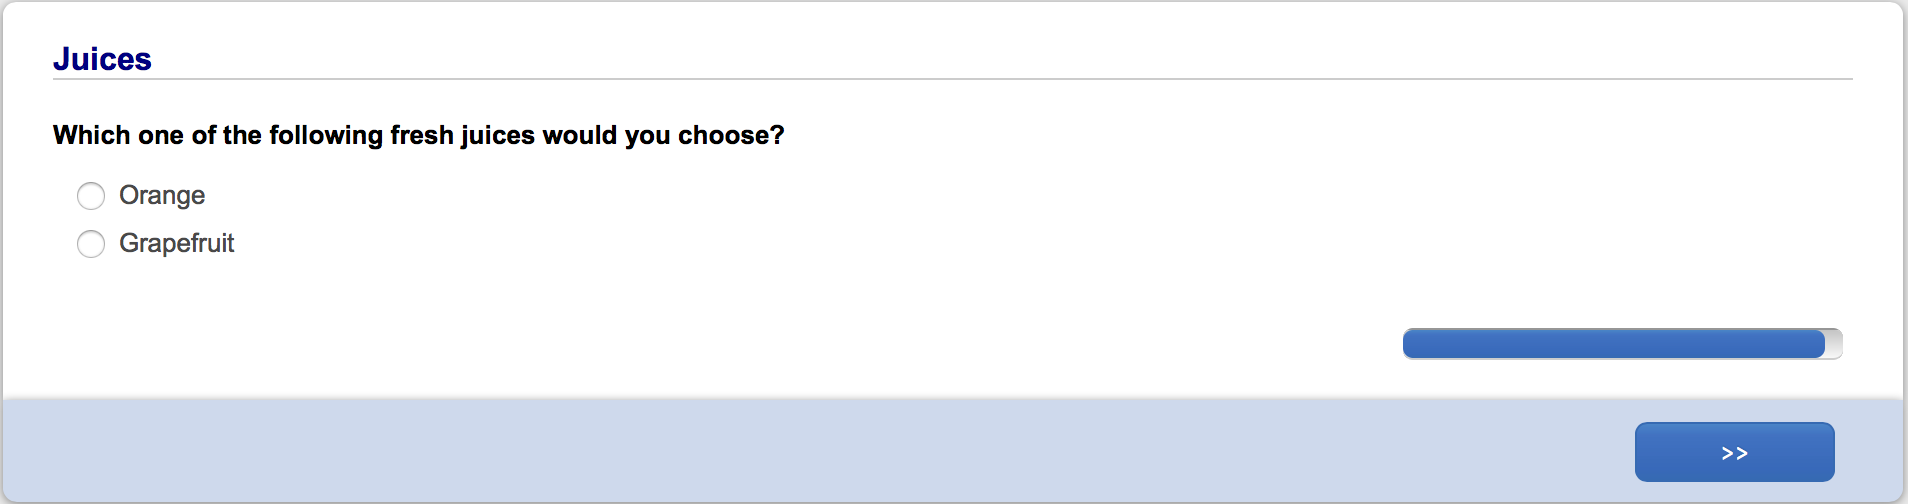
\includegraphics[width=15cm]{Population_study_design/screenshot_juices.png}

\subsubsection*{Observed binary and ternary choices}

\includegraphics[width=15cm]{./Population_study_data/Simplexes/juices.pdf}

\pagebreak

\subsection*{Colours}
%%%%%%%%%%%%%%%%%%%%

% Colours

\begin{tcolorbox}
Which one of the following colours do you like best?

\begin{itemize}
	\setlength\itemsep{-5pt}
	\item Red
	\item Purple
	\item Pink
	\item Blue
	\item Green
\end{itemize}
\end{tcolorbox}


\subsubsection*{Random screenshot}

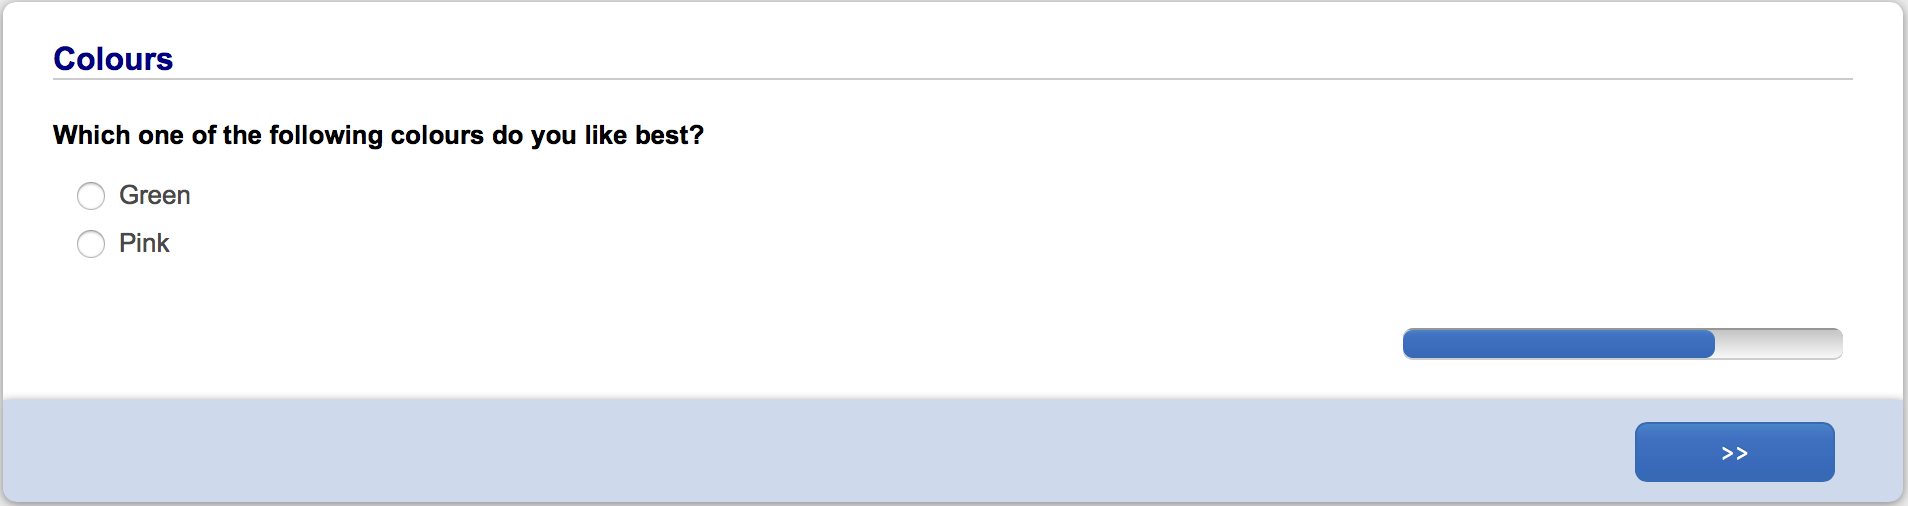
\includegraphics[width=15cm]{Population_study_design/screenshot_colours.png}

\subsubsection*{Observed binary and ternary choices}

\includegraphics[width=15cm]{./Population_study_data/Simplexes/colours.pdf}

\pagebreak

\subsection*{Color pairs}
%%%%%%%%%%%%%%%%%%%%%%%%

% Colour pairs

The source for this domain is the website ``The top tens'', page ``Two colors that look good side by side.''
The color combinations here are ranked 1, 4, 5, 13 and 14.
We chose a selection of five high ranking combinations among which there were many colors
in common.
Using a similarity measure equal to the number of colours in common between two pairs, there are two doubleton choice sets where the two colour pairs have no colours in common ($\{a,e\}$ and $\{b,d\}$) and eight where the two colour pairs have one colour in common.
This gives six tripleton pairs in which one might expect a similarity effect.

\begin{tcolorbox}
Which one of these colour combinations do you like best?

\begin{itemize}
	\setlength\itemsep{-5pt}
	\item Black and red
	\item Black and purple
	\item Black and blue
	\item Blue and red
	\item Blue and purple
\end{itemize}
\end{tcolorbox}


\subsubsection*{Random screenshot}

\includegraphics[width=15cm]{Population_study_design/screenshot_colour_pairs.png}

\subsubsection*{Observed binary and ternary choices}

\includegraphics[width=15cm]{./Population_study_data/Simplexes/colour_pairs.pdf}

\pagebreak

\subsection*{Events}
%%%%%%%%%%%%%%%%%%%

% Events

This domain involves comparisons of the probabilities of future events.
Logically, the probability of event e must be as least as great as the probability of a, which must in turn be as least as great as the probability of d; also, the probability of b must be at least as great as the probability of c.
There is potential for several asymmetric dominance effects in this domain, based on these dominance relations.
These would be unconventional effets, as most experimental designs in the literature intended to elicit asymmetric dominance effects feature numerical dominance relations.

\begin{tcolorbox}
Which one of the following events do you think is most likely to happen in the next twenty years?

\begin{itemize}
	\setlength\itemsep{-5pt}
	\item Scotland becomes an independent country.
	\item Either Catalonia or Quebec become independent countries.
	\item Catalonia becomes an independent country.
	\item Scotland and Quebec become independent countries.
	\item Either Scotland or Quebec become independent countries.
\end{itemize}
\end{tcolorbox}


\subsubsection*{Random screenshot}

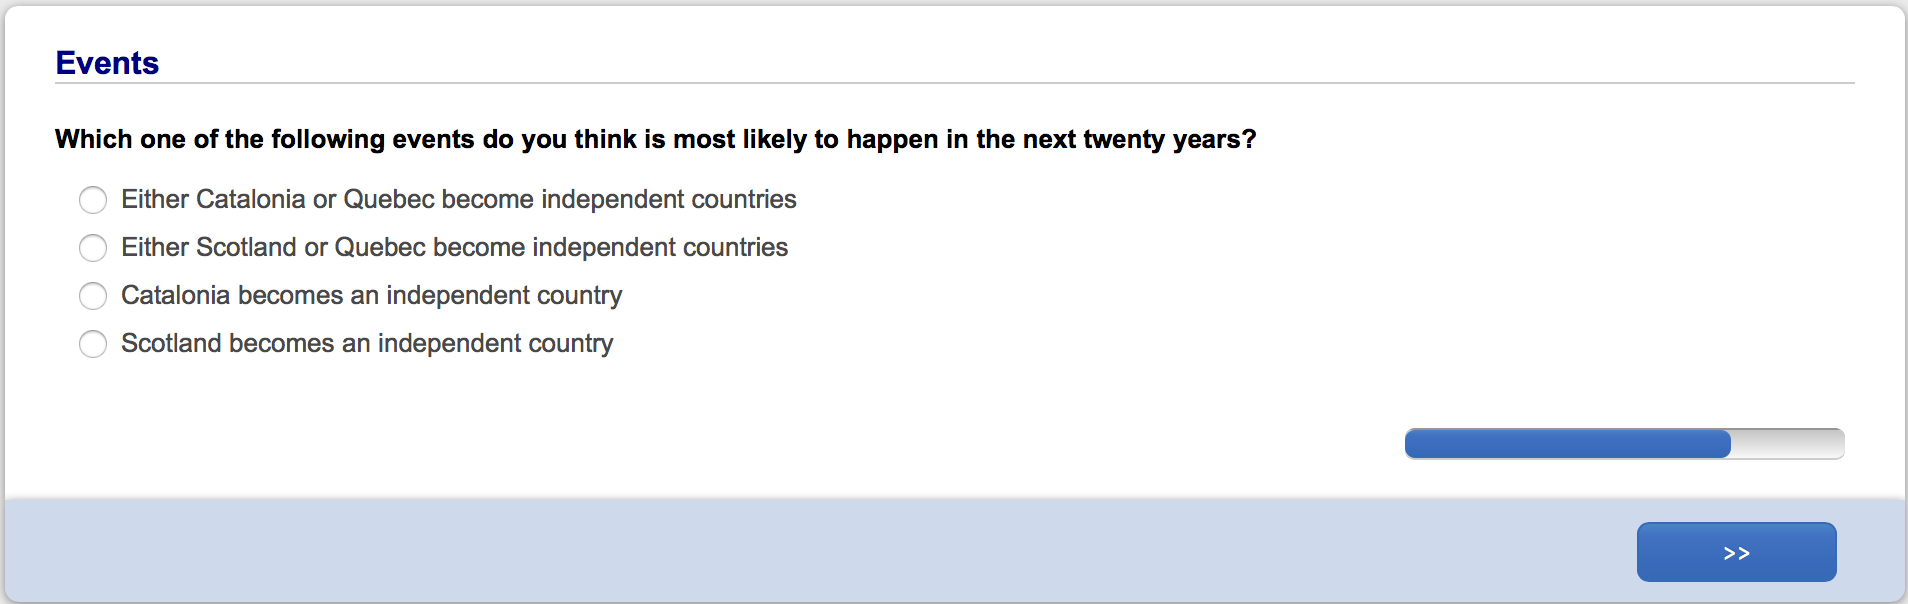
\includegraphics[width=15cm]{Population_study_design/screenshot_events.png}

\subsubsection*{Observed binary and ternary choices}

\includegraphics[width=15cm]{./Population_study_data/Simplexes/events.pdf}

\pagebreak

\subsection*{Radio formats}
%%%%%%%%%%%%%%%%%%%%%%%%%%

% Radio formats

The domain is radio formats, and the choice objects are the top 5 radio formats in Canada in 2015, according to
\begin{quotation}
	https://byrnesmedia.com/2015/10/05/the-6-best-performing-radio-formats-in-canada/
\end{quotation}
Descriptions of formats are from
\begin{quotation}
	http://www.newsgeneration.com/broadcast-resources/guide-to-radio-station-formats/
\end{quotation}

\begin{tcolorbox}
Suppose you were on a two hour road trip and you have a choice among radio stations with the following formats.
Which one would you choose?

\begin{itemize}
	\setlength\itemsep{-5pt}
	\item News
	\item Hot Adult Contemporary, or Hot AC
	(A variety of classic and contemporary mainstream music geared towards adults.)
	\item Classic Hits (Rock and pop, roughly 1964-1989)
	\item Country Music
	\item Adult Contemporary, or AC (Adult-oriented pop/rock with no hard rock.)
\end{itemize}
\end{tcolorbox}


\subsubsection*{Random screenshot}

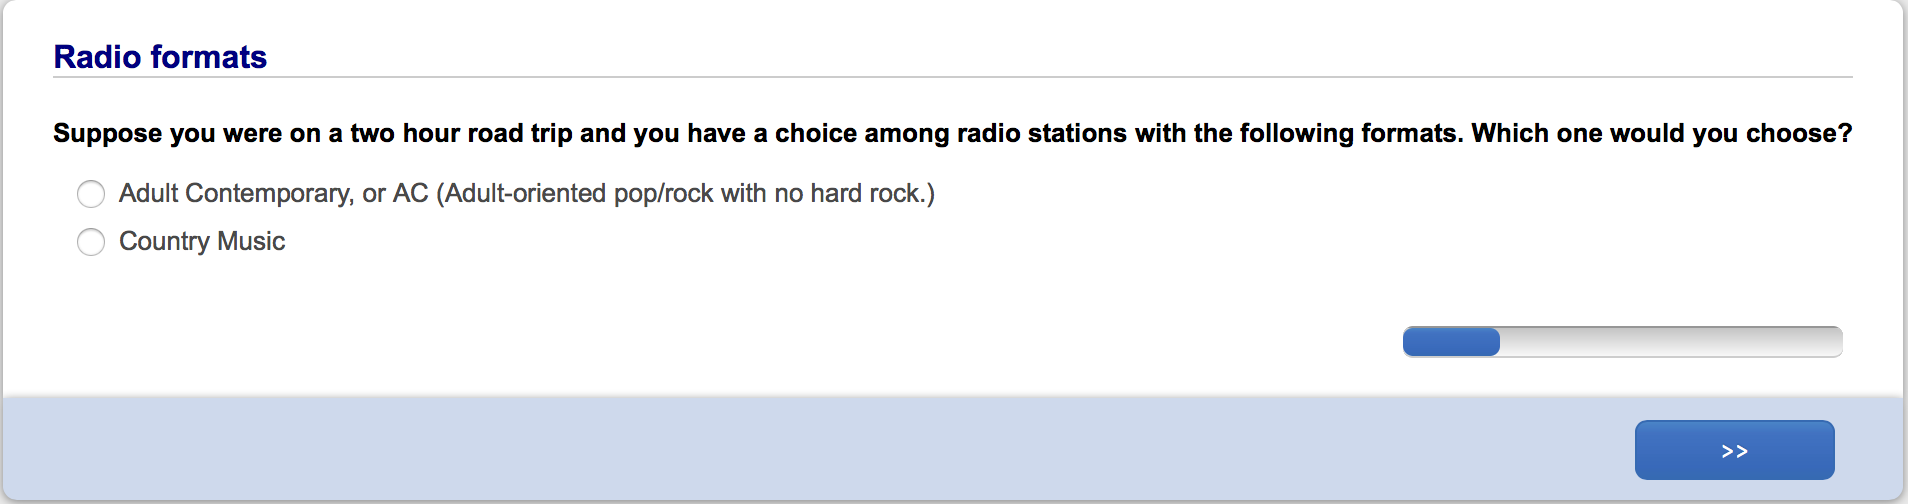
\includegraphics[width=15cm]{Population_study_design/screenshot_radio.png}

\subsubsection*{Observed binary and ternary choices}

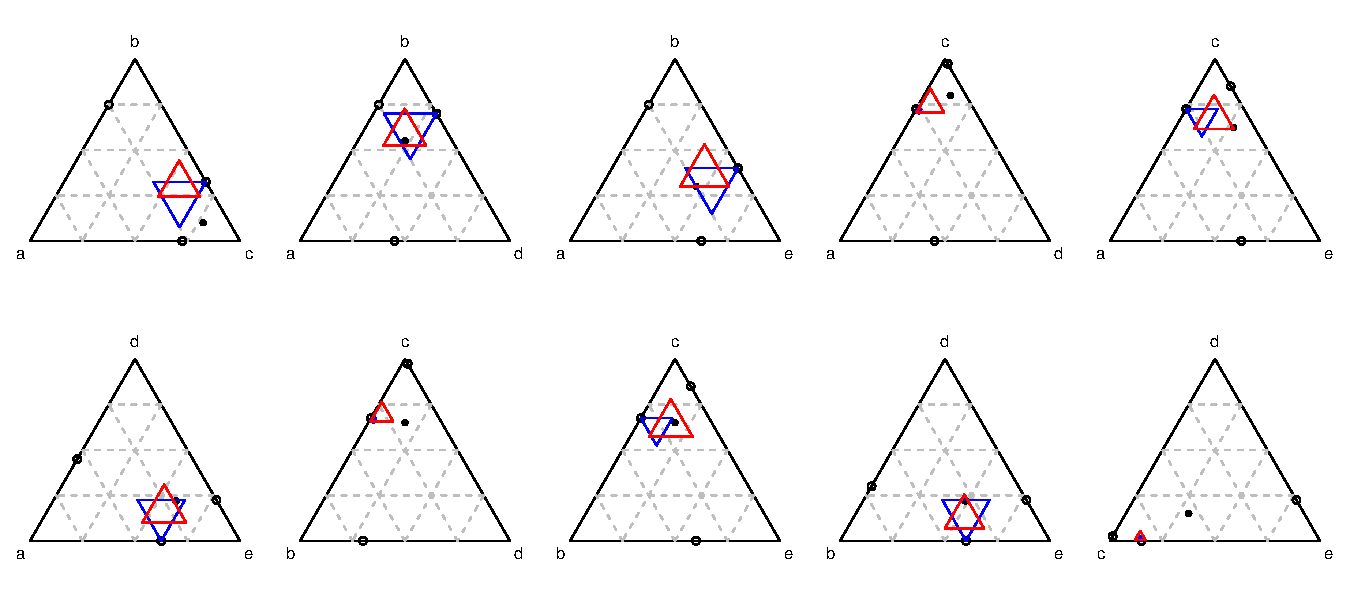
\includegraphics[width=15cm]{./Population_study_data/Simplexes/radio.pdf}

\pagebreak

\subsection*{Musical artists}
%%%%%%%%%%%%%%%%%%%%%%%%%%%%

% Musical artists

The choice objects in this domain are the top selling musical artists of all time, according to Wikipedia.
They should be familiar to a large majority of respondents.

\begin{tcolorbox}
Which one of the following musical artists do you like the best?

\begin{itemize}
	\setlength\itemsep{-5pt}
	\item The Beatles
	\item Elvis Presley
	\item Michael Jackson
	\item Madonna
	\item Elton John
\end{itemize}
\end{tcolorbox}


\subsubsection*{Random screenshot}

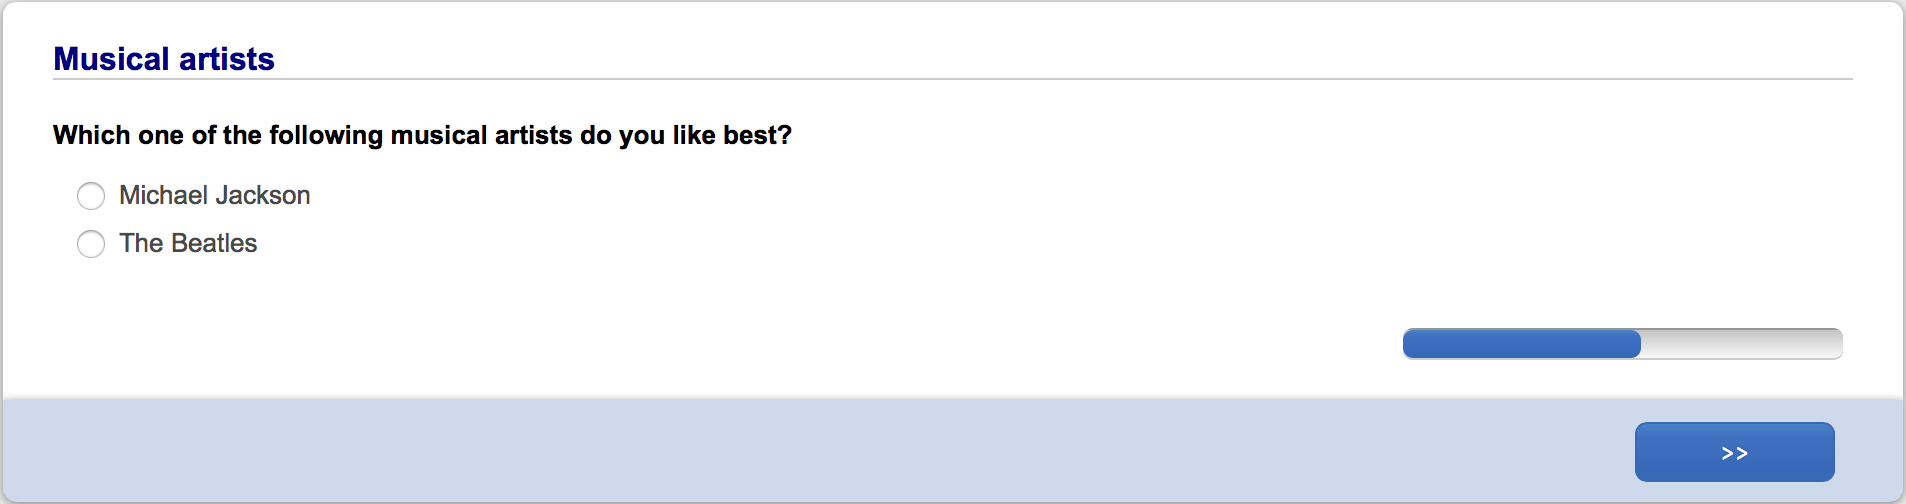
\includegraphics[width=15cm]{Population_study_design/screenshot_music.png}

\subsubsection*{Observed binary and ternary choices}

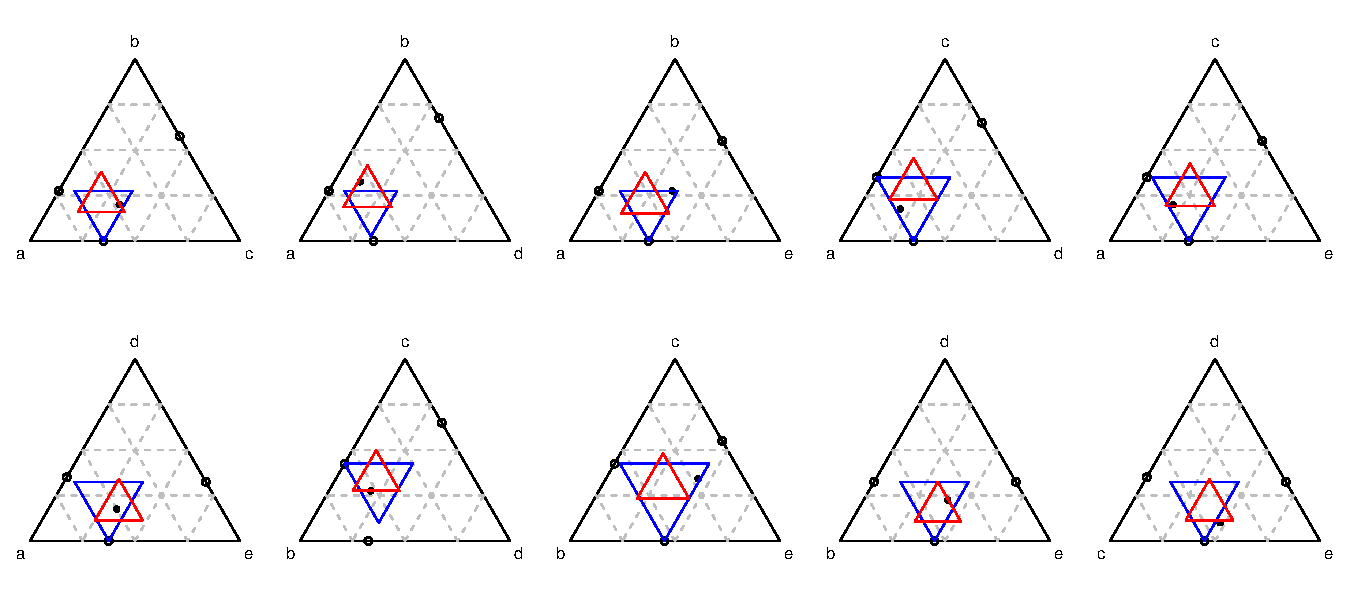
\includegraphics[width=15cm]{./Population_study_data/Simplexes/music.pdf}

\pagebreak

\subsection*{Aboriginal art}
%%%%%%%%%%%%%%%%%%%%%%%%%%%

% Aboriginal art

\begin{tcolorbox}
Which one of the following examples of Australian aboriginal art do you like the best?

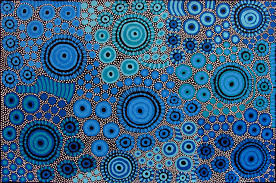
\includegraphics[width=3cm]{Population_study_design/Aboriginal_art1.jpg}
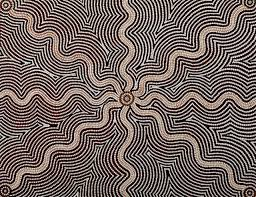
\includegraphics[width=3cm]{Population_study_design/Aboriginal_art2.jpg}
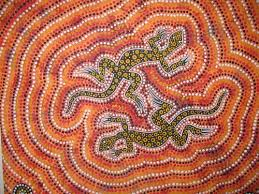
\includegraphics[width=3cm]{Population_study_design/Aboriginal_art3.jpg}

\includegraphics[width=3cm]{Population_study_design/Aboriginal_art4.jpg}

\includegraphics[width=3cm]{Population_study_design/Aboriginal_art5.jpg}
\end{tcolorbox}


\subsubsection*{Random screenshot}

\includegraphics[width=15cm]{Population_study_design/screenshot_aboriginal_art.png}

\subsubsection*{Observed binary and ternary choices}

\includegraphics[width=15cm]{./Population_study_data/Simplexes/aboriginal_art.pdf}

\pagebreak

\subsection*{Impressionist art}
%%%%%%%%%%%%%%%%%%%%%%%%%%%%%%

% Impressionist Art

\begin{tcolorbox}
Which one of the following examples of Impressionist art do you like the best?

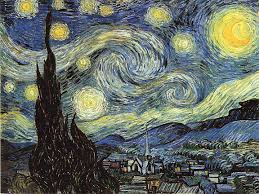
\includegraphics[width=3cm]{Population_study_design/Impressionist_art1.jpg}
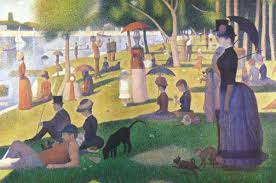
\includegraphics[width=3cm]{Population_study_design/Impressionist_art2.jpg}
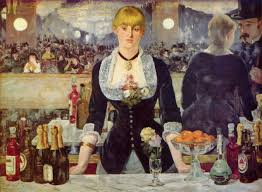
\includegraphics[width=3cm]{Population_study_design/Impressionist_art3.jpg}
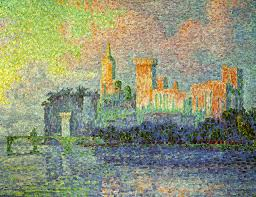
\includegraphics[width=3cm]{Population_study_design/Impressionist_art4.jpg}
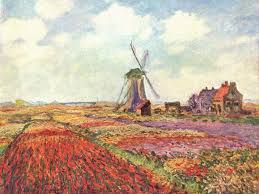
\includegraphics[width=3cm]{Population_study_design/Impressionist_art5.jpg}
\end{tcolorbox}


\subsubsection*{Random screenshot}

\includegraphics[width=15cm]{Population_study_design/screenshot_impressionist_art.png}

\subsubsection*{Observed binary and ternary choices}

\includegraphics[width=15cm]{./Population_study_data/Simplexes/impressionist_art.pdf}

\pagebreak

\subsection*{Sentences}
%%%%%%%%%%%%%%%%%%%%%%

% Sentences

This domain consists of sentences that have been used in experiments of linguistic judgement.
They are, respectively sentences 7j, 7h, 7p, 7a and 7e in \citeasnoun{BardRobeSora96}.
Figure 1 of that paper shows acceptability scores for these and other sentences given by two individual linguists, an acceptability score aggregating the scores of four linguists and an acceptability score aggregating the scores of four ``naive respondents'', all undergraduate anatomy students.
There is broad, but not perfect, agreement in terms of order, and in the following list, they are in decreasing order of acceptability according to the measure aggregating the judgements of four linguists.

\begin{tcolorbox}
Which one of the following sentences do you find the most grammatically acceptable?

\begin{itemize}
	\setlength\itemsep{-5pt}
	\item Who did Bill buy the car to please?
	\item This is a book which reading would be fun.
	\item Where did Bill buy the car to drive?
	\item Which man do you wonder when to meet?
	\item With which pen do you wonder what to write?
\end{itemize}
\end{tcolorbox}


\subsubsection*{Random screenshot}

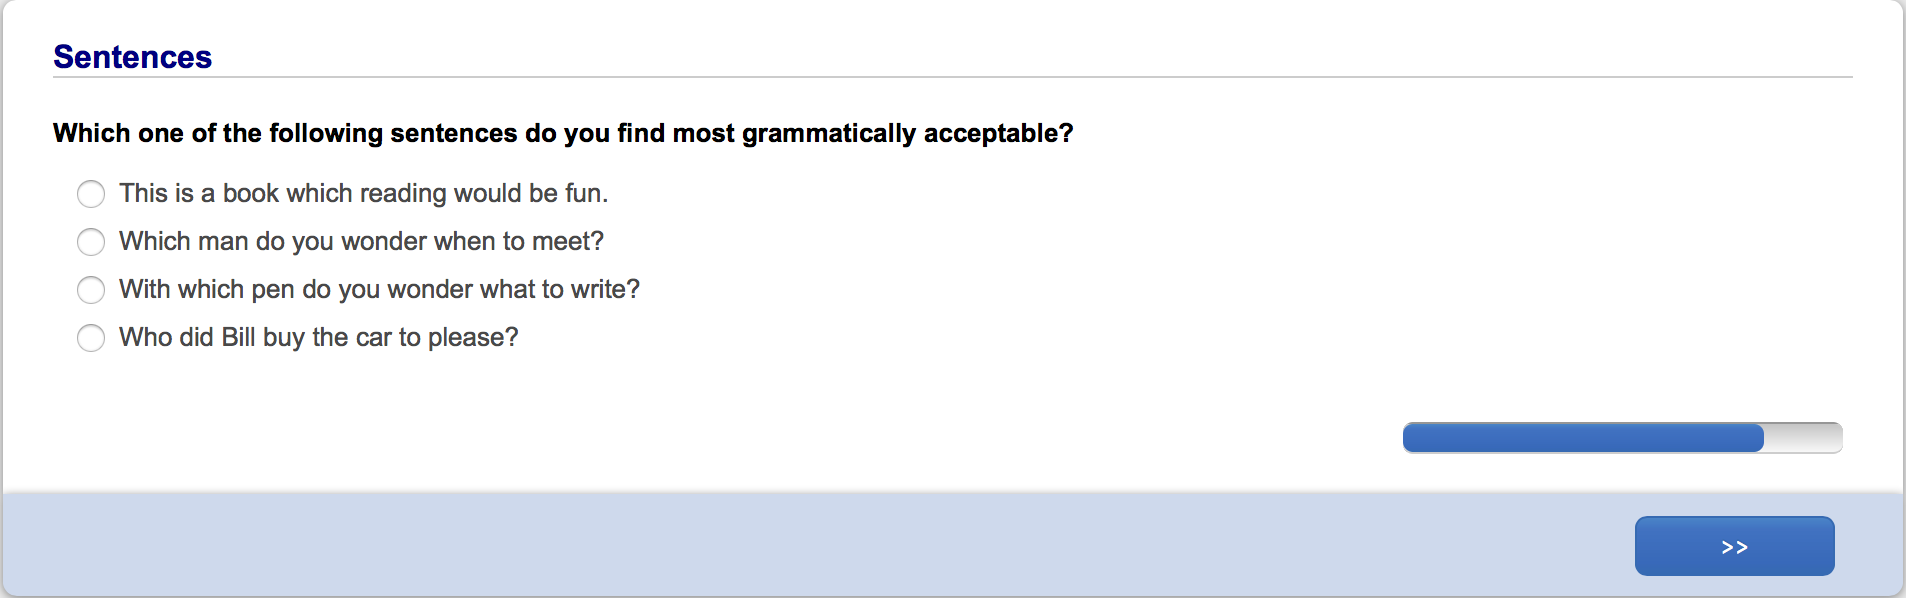
\includegraphics[width=15cm]{Population_study_design/screenshot_sentences.png}

\subsubsection*{Observed binary and ternary choices}

\includegraphics[width=15cm]{./Population_study_data/Simplexes/sentences.pdf}

\pagebreak

\subsection*{Travel}
%%%%%%%%%%%%%%%%%%%

% Travel

The source is Tripadvisor.
These are the top five travel destinations, according to the results of an on-line contest where visitors to a Tripadvisor site could make pairwise choices between travel destinations.

\begin{tcolorbox}
\begin{quotation}
Which one of the following travel destinations would you most like to visit?
\end{quotation}

\begin{enumerate}
\item Marrakech, Morocco
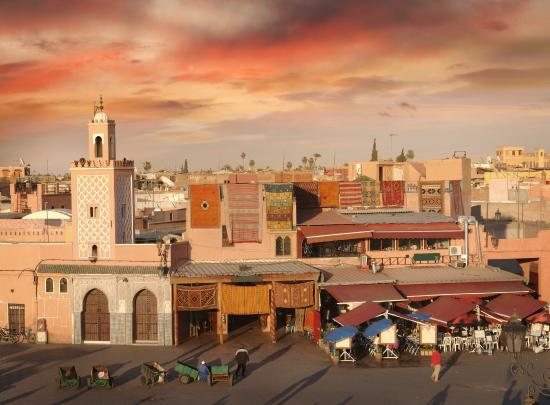
\includegraphics[height=2.8cm]{Population_study_design/Travel1.jpg}

\item Istanbul, Turkey
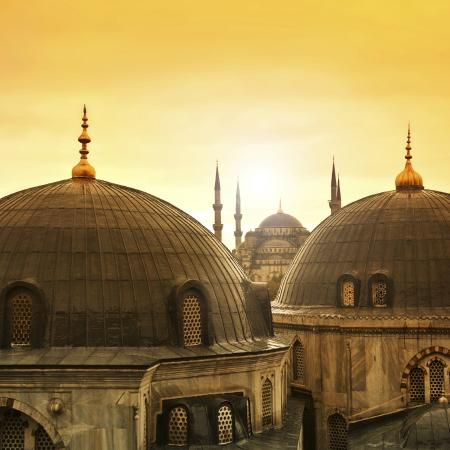
\includegraphics[height=2.8cm]{Population_study_design/Travel2.jpg}

\item Hanoi, Vietnam
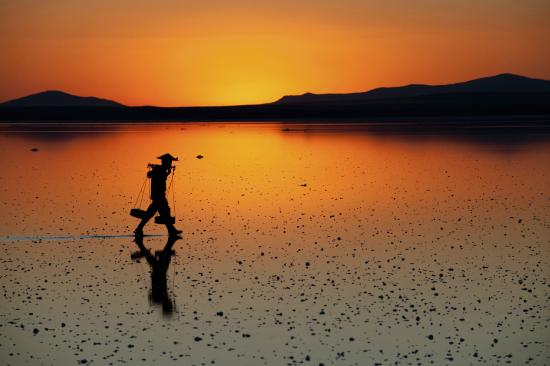
\includegraphics[height=2.8cm]{Population_study_design/Travel3.jpg}

\item Siem Reap, Cambodia
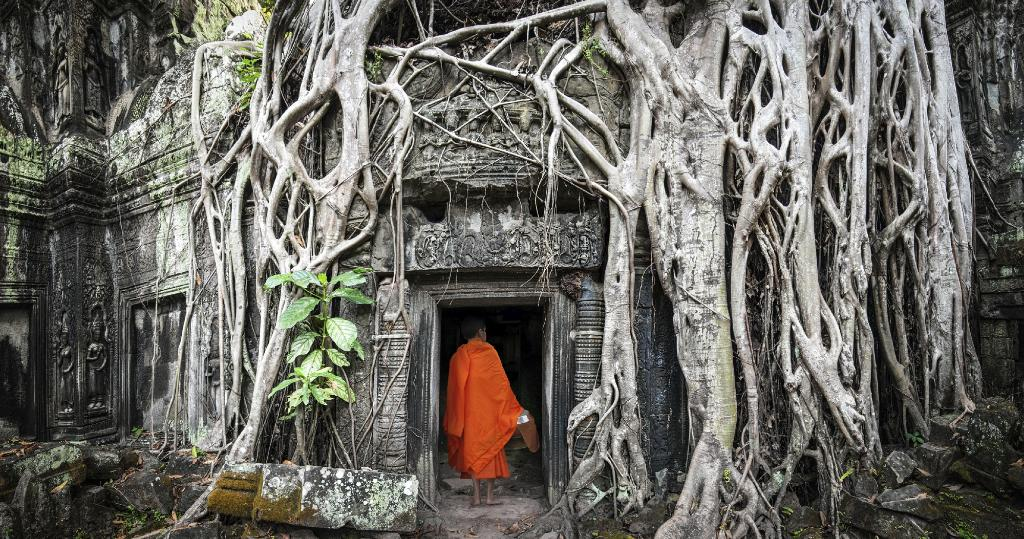
\includegraphics[height=2.8cm]{Population_study_design/Travel4.jpg}

\item Praque, Czech Republic
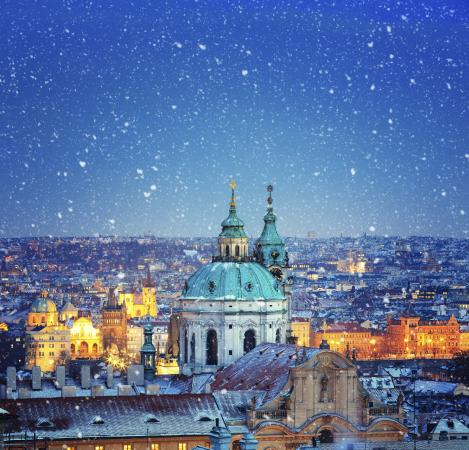
\includegraphics[height=2.8cm]{Population_study_design/Travel5.jpg}
\end{enumerate}	
\end{tcolorbox}


\subsubsection*{Random screenshot}

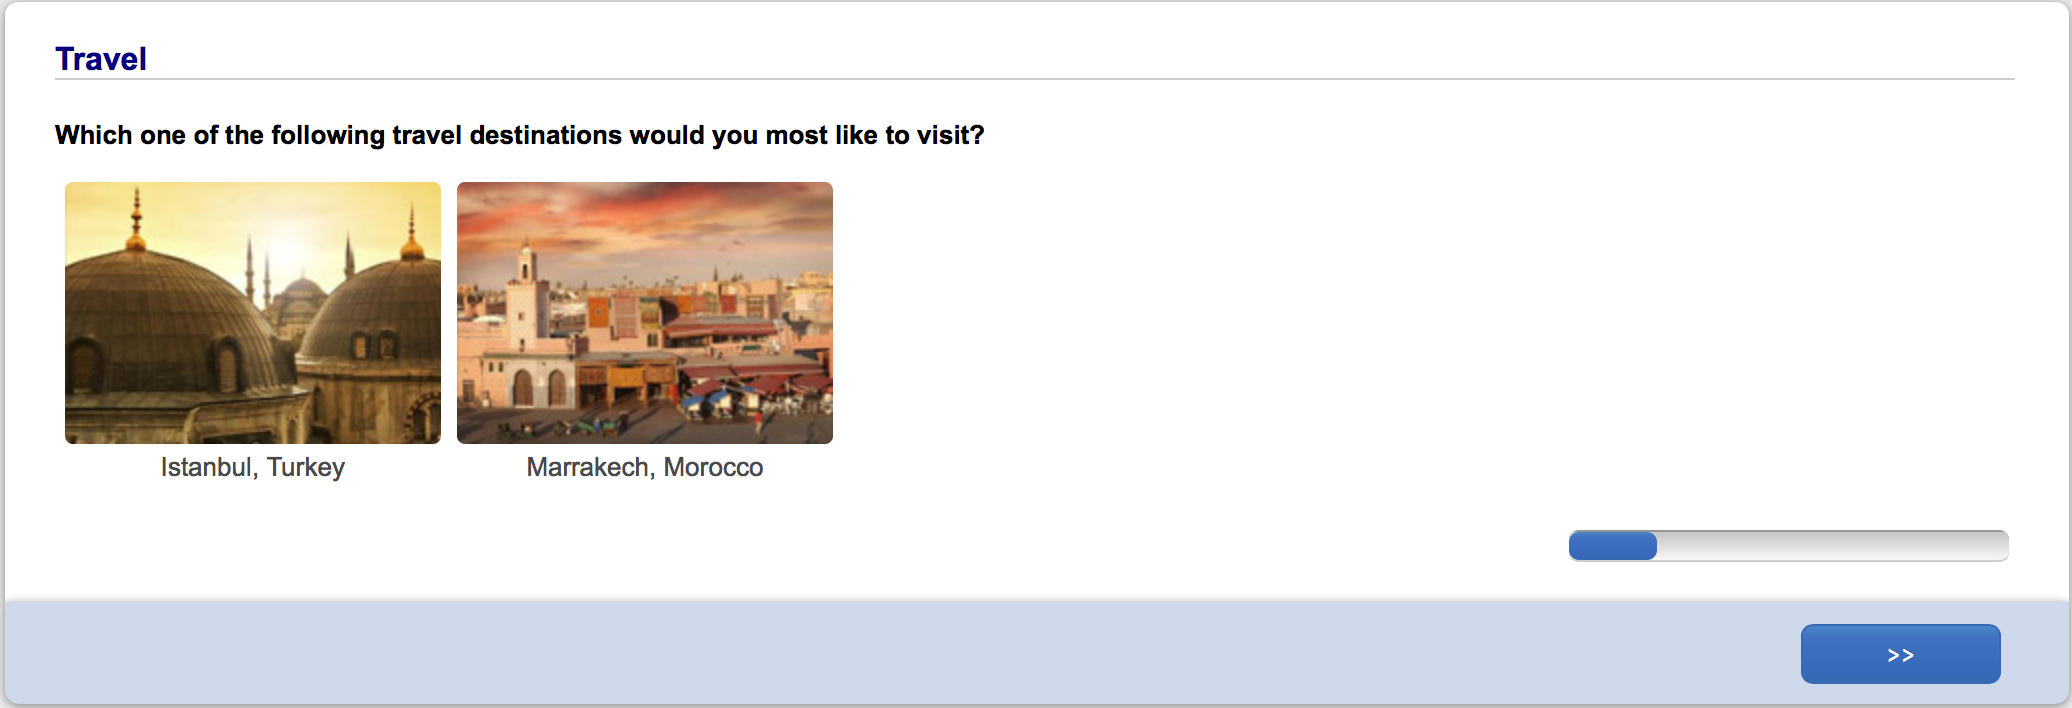
\includegraphics[width=15cm]{Population_study_design/screenshot_travel.png}

\subsubsection*{Observed binary and ternary choices}

\includegraphics[width=15cm]{./Population_study_data/Simplexes/travel.pdf}

\pagebreak

\subsection*{Marijuana}
%%%%%%%%%%%%%%%%%%%%%%

% Marijuana

This question elicits policy preferences.

\begin{tcolorbox}
Which one of the following marijuana policies would you choose?

\begin{itemize}
	\setlength\itemsep{-5pt}
	\item Possession by, and sales to adults are both legal; sales to minors are illegal.
	\item Possession by, and sales to adults are both illegal but neither is a criminal offense; sales to minors are a criminal offense.
	\item Possession is illegal but not criminal; all sales are a criminal offense.
	\item Possession and sales are criminal offenses, with a small number of medical exceptions.
	\item Possession and sales are criminal offenses, without exception.
\end{itemize}
\end{tcolorbox}


\subsubsection*{Random screenshot}

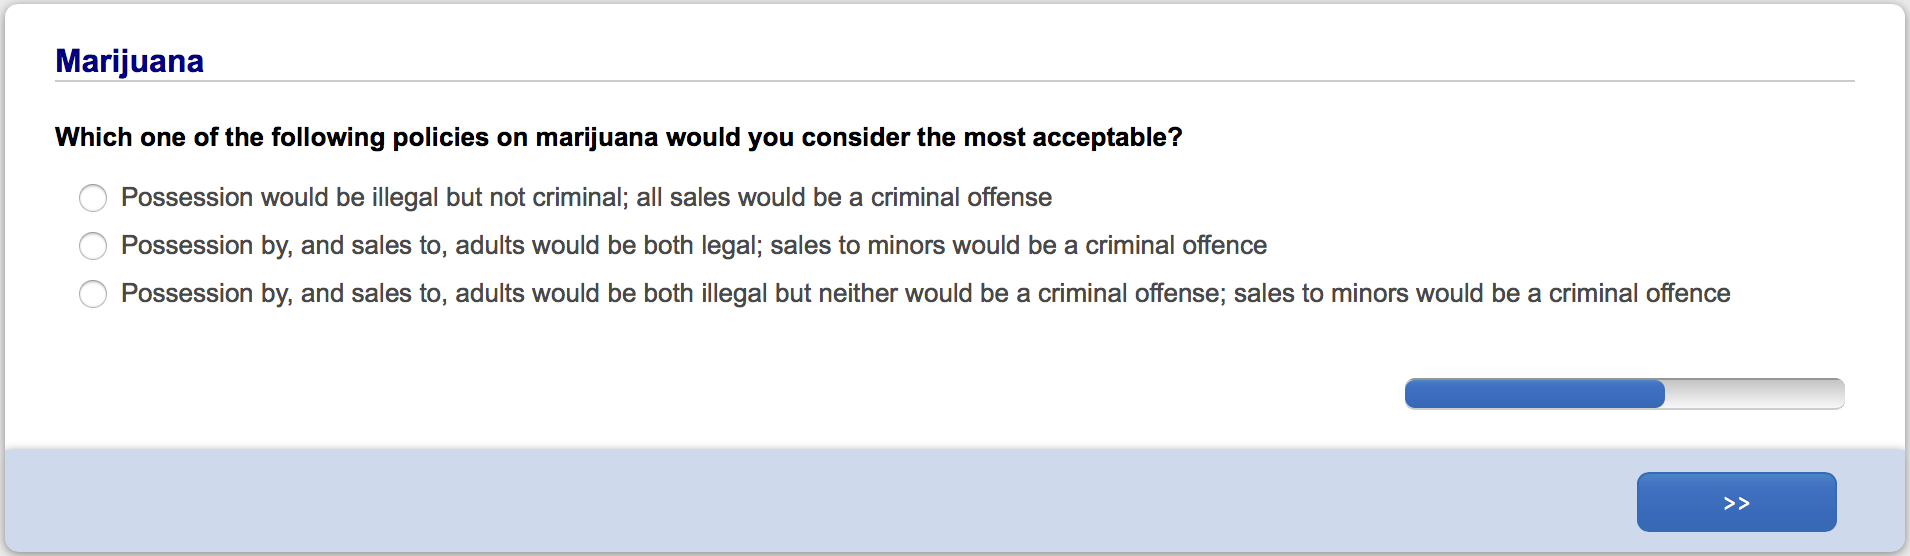
\includegraphics[width=15cm]{Population_study_design/screenshot_marijuana.png}

\subsubsection*{Observed binary and ternary choices}

\includegraphics[width=15cm]{./Population_study_data/Simplexes/marijuana.pdf}

\pagebreak

\subsection*{Latitude}
%%%%%%%%%%%%%%%%%%%%%

% Latitude

The five cities of this domain have a latitude close to 50 degrees north.
In the following list, they are ordered from furthest north to furthest south.
According to Wikipedia, their latitudes are, respectively, $52\degree14^\prime N$, $51\degree30^\prime N$, $49\degree15^\prime N$, $48\degree51^\prime N$ and $47\degree36^\prime N$.
There are two potential asymmetric dominance effects, with Vancouver being fairly obviously north of Seattle and London being fairly obviously north of Paris.

\begin{tcolorbox}
Which one of the following cities do you think is furthest north?

\begin{itemize}
	\setlength\itemsep{-5pt}
	\item Warsaw, Poland
	\item London, United Kingdom
	\item Vancouver, Canada
	\item Paris, France
	\item Seattle, United States
\end{itemize}
\end{tcolorbox}


\subsubsection*{Random screenshot}

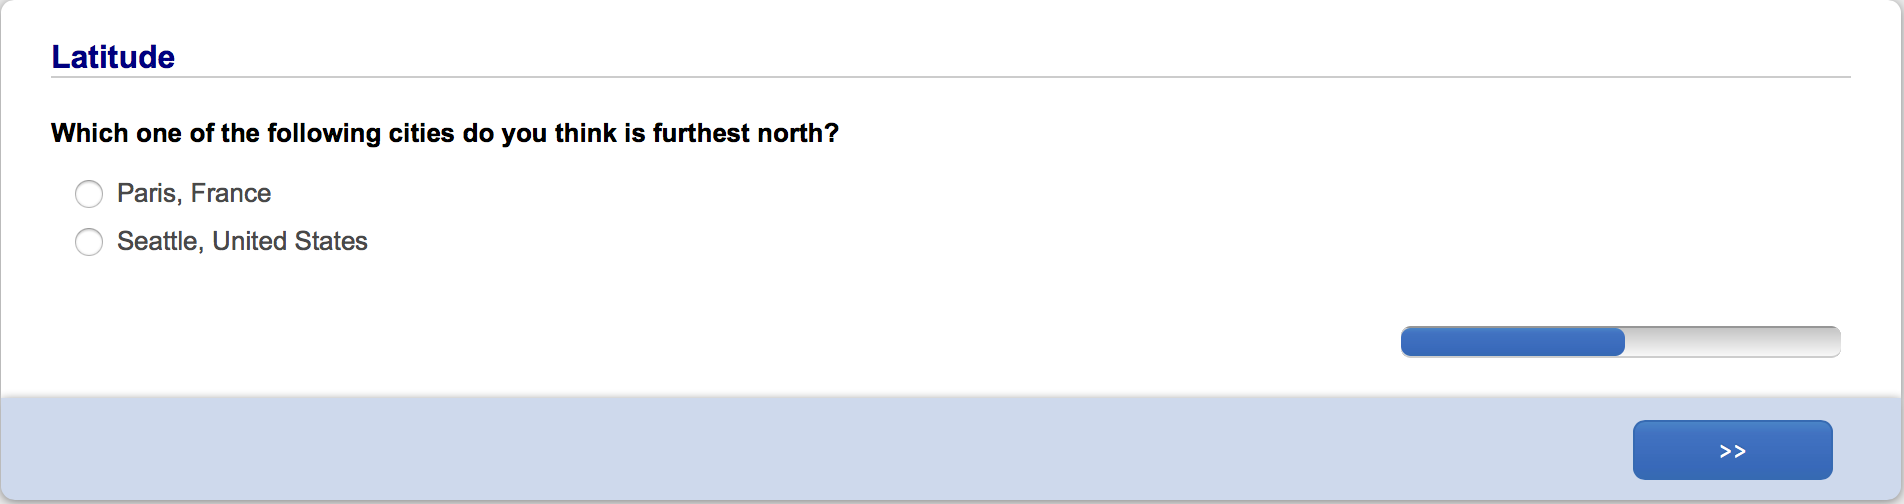
\includegraphics[width=15cm]{Population_study_design/screenshot_latitude.png}

\subsubsection*{Observed binary and ternary choices}

\includegraphics[width=15cm]{./Population_study_data/Simplexes/latitude.pdf}

\pagebreak

\subsection*{Scatterplots}
%%%%%%%%%%%%%%%%%%%%%%%%%

% Dots

This domain is a perception example.
The true numbers of points are, respectively, 320, 310, 300, 290 and 280.
It is much clearer that there are more points in the first panel than in the fifth, than that there are more points in the first than in the second.
The difference in the number of points is an obvious similarity measure here that might be expected to lead to similarity effects.
{}
\begin{tcolorbox}
Which one of the following boxes do you think has the greatest number of points?

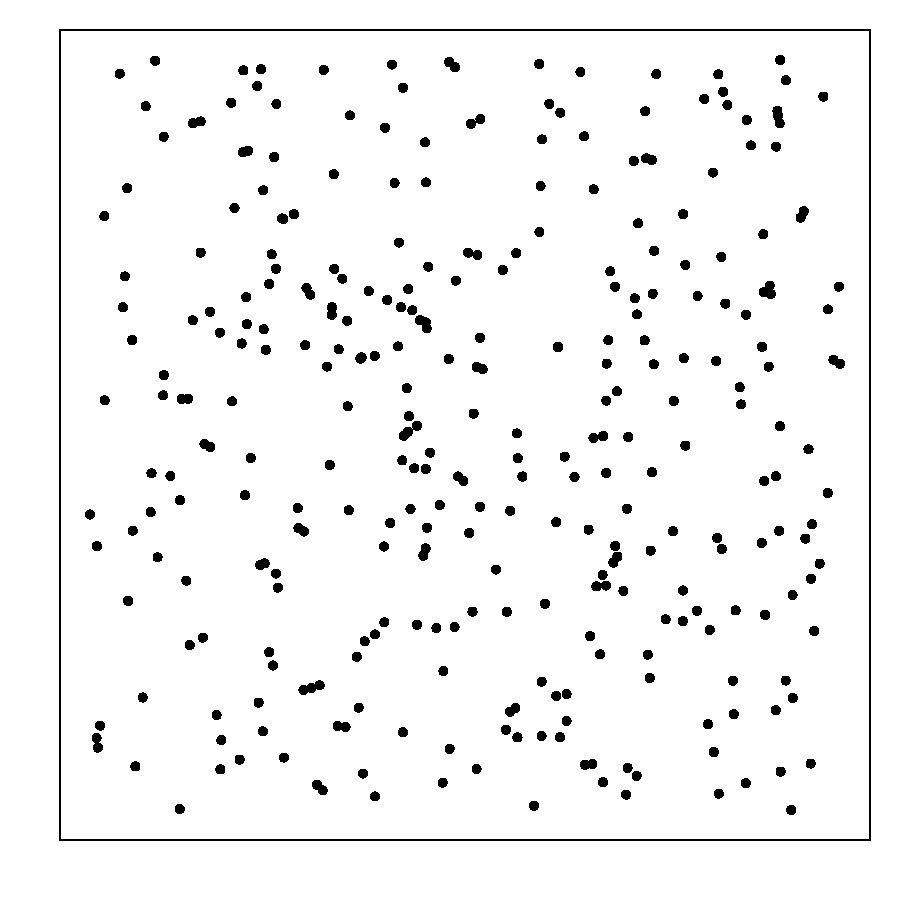
\includegraphics[height=3cm]{Population_study_design/Scatterplots1.pdf}
\includegraphics[height=3cm]{Population_study_design/Scatterplots2.pdf}
\includegraphics[height=3cm]{Population_study_design/Scatterplots3.pdf}
\includegraphics[height=3cm]{Population_study_design/Scatterplots4.pdf}
\includegraphics[height=3cm]{Population_study_design/Scatterplots5.pdf}
\end{tcolorbox}


\subsubsection*{Random screenshot}

\includegraphics[width=15cm]{Population_study_design/screenshot_dots.png}

\subsubsection*{Observed binary and ternary choices}

\includegraphics[width=15cm]{./Population_study_data/Simplexes/dots.pdf}

\pagebreak

\subsection*{Triangles}
%%%%%%%%%%%%%%%%%%%%%%

% Triangles

This domain is another perception example.
The true areas are, respectively, 16, 15, 15, 14 and 14 units.

\begin{tcolorbox}
	Which one of the following triangles do you think has the greatest area?

	\includegraphics[height=3cm]{Population_study_design/Triangles3.pdf}
	\includegraphics[height=3cm]{Population_study_design/Triangles1.pdf}
	\includegraphics[height=3cm]{Population_study_design/Triangles2.pdf}
	\includegraphics[height=3cm]{Population_study_design/Triangles4.pdf}
	\includegraphics[height=3cm]{Population_study_design/Triangles5.pdf}	
\end{tcolorbox}


\subsubsection*{Random screenshot}

\includegraphics[width=15cm]{Population_study_design/screenshot_triangles.png}

\subsubsection*{Observed binary and ternary choices}

\includegraphics[width=15cm]{./Population_study_data/Simplexes/triangles.pdf}

\pagebreak

\subsection*{Population}
%%%%%%%%%%%%%%%%%%%%%%%

% Population

These countries were ranked, respectively, 4th through 8th in terms of population in 2016, when
their populations, in millions, were 258, 206, 202, 186 and 156.

\begin{tcolorbox}
Which one of the following countries do you think has the largest population?

\begin{itemize}
	\setlength\itemsep{-5pt}
	\item Indonesia
	\item Brazil
	\item Pakistan
	\item Nigeria
	\item Bangladesh
\end{itemize}
\end{tcolorbox}


\subsubsection*{Random screenshot}

\includegraphics[width=15cm]{Population_study_design/screenshot_population.png}

\subsubsection*{Observed binary and ternary choices}

\includegraphics[width=15cm]{./Population_study_data/Simplexes/population.pdf}

\pagebreak

\subsection*{Surface area}
%%%%%%%%%%%%%%%%%%%%%%%%%

% Surface area

These countries are ranked, respectively, 2nd through 6th in terms of surface area, including inland bodies of water.
In millions of square kilometres, those surface areas are 9.984, 9.573, 9.525, 8.516 and 7.692.

\begin{tcolorbox}
Which one of the following countries do you think has the greatest surface area, including inland bodies of water?
	
\begin{itemize}
	\setlength\itemsep{-5pt}
	\item Canada
	\item United States of America
	\item China
	\item Brazil
	\item Australia
\end{itemize}
\end{tcolorbox}


\subsubsection*{Random screenshot}

\includegraphics[width=15cm]{Population_study_design/screenshot_area.png}

\subsubsection*{Observed binary and ternary choices}

\includegraphics[width=15cm]{./Population_study_data/Simplexes/area.pdf}

\pagebreak

\subsection*{Beer}
%%%%%%%%%%%%%%%%%

% Beer

This domain is from an experiment reported in \citeasnoun{HubePaynPuto82} used to illustrate an asymmetric dominance effect.
The prices are multiplied by 5 and we added choice objects d and e to allow for two more asymmetric dominance effects and two similarity effects.
The first panel of Figure \ref{f:CE} show the choice objects in attribute space.
Table \ref{t:CE} shows the relations of dominance, similarity and betweenness among objects associated with context effects.
The most commonly used domains to illustrate the attraction effect involve Beer, Cars, Apartments, Computers, Restaurants and Televisions.

\begin{tcolorbox}
Below you will find three brands of beer.
You know only the price per sixpack and the average quality ratings made by respondents in a blind taste test.
Given that you had to choose one brand to buy on this information alone, which one would you choose?

\begin{tabular}{cc}
\hline
Price/sixpack & Average quality rating (100 = Best; 0 = Worst) \\ 
\hline
\$9.00 & 50 \\ 
\$13.00 & 70 \\ 
\$15.00 & 70 \\ 
\$14.00 & 75 \\ 
\$15.00 & 80 \\ \hline
\end{tabular}
\end{tcolorbox}


\subsubsection*{Random screenshot}

\includegraphics[width=15cm]{Population_study_design/screenshot_beer.png}

\subsubsection*{Observed binary and ternary choices}

\includegraphics[width=15cm]{./Population_study_data/Simplexes/beer.pdf}

\pagebreak

\subsection*{Cars}
%%%%%%%%%%%%%%%%%

% Cars

This domain is based on an experiment from \citeasnoun{WedePett96}.
There are two experiments involving cars in that article, the experiment in question is  numbered 18 in the appendix to that paper.
Objects below have the same attributes as in that experiment and a similar range of levels.
We adapted the objects to allow for compromise effects.
The second panel of Figure \ref{f:CE} shows the choice objects in attribute space.
Table \ref{f:CE} shows the relations of dominance, similarity and betweenness among objects associated with context effects.

\begin{tcolorbox}
Which one of the following cars would you choose to drive, all other features
begin equal? Ride quality is a on a scale of 0 to 100.

\begin{tabular}{cc}
\hline
Ride quality & Miles per gallon \\ \hline
60 & 30 \\ 
80 & 24 \\ 
70 & 27 \\ 
55 & 28 \\ 
75 & 22 \\ \hline
\end{tabular}
\end{tcolorbox}


\subsubsection*{Random screenshot}

\includegraphics[width=15cm]{Population_study_design/screenshot_cars.png}

\subsubsection*{Observed binary and ternary choices}

\includegraphics[width=15cm]{./Population_study_data/Simplexes/cars.pdf}

\pagebreak

\subsection*{Restaurants}
%%%%%%%%%%%%%%%%%%%%%%%%

% Restaurants

This domain is based on another experiment in \citeasnoun{WedePett96}, numbered 19 in the appendix to that paper.
The third panel of Figure \ref{f:CE} shows the choice objects in attribute space.
Table \ref{t:CE} shows the relations of dominance, similarity and betweenness among objects associated with context effects.

\begin{tcolorbox}
Which one of the following restaurants would you choose for your next restaurant meal, based on transportation time (in minutes) and average customer ratings (from
1 to 5).
	
\begin{tabular}{cc}
\hline
Transportation time & Rating \\ \hline
34 & 4.4 \\ 
22 & 4.0 \\ 
19 & 3.9 \\ 
7 & 3.5 \\ 
22 & 3.9 \\ \hline
\end{tabular}
\end{tcolorbox}


\subsubsection*{Random screenshot}

\includegraphics[width=15cm]{Population_study_design/screenshot_restaurants.png}

\subsubsection*{Observed binary and ternary choices}

\includegraphics[width=15cm]{./Population_study_data/Simplexes/restaurants.pdf}

\pagebreak

\subsection*{Layovers}
%%%%%%%%%%%%%%%%%%%%%%%%%%%%

% Layovers

The fourth panel of Figure \ref{f:CE} shows the choice objects in attribute space.
Table \ref{t:CE} shows the relations of dominance, similarity and betweenness among objects associated with context effects.

\begin{tcolorbox}
Which one of the following flight itineraries would you choose?
All involve two flights, with one layover between them.

\begin{tabular}{ccc}
\hline
Total inflight time & Layover time & Total itinerary time \\ \hline
4:00 & 1:00 & 5:00 \\ 
3:24 & 1:48 & 5:12 \\ 
3:15 & 2:00 & 5:15 \\ 
3:06 & 2:12 & 5:18 \\ 
2:30 & 3:00 & 5:30 \\ \hline
\end{tabular}
\end{tcolorbox}


\subsubsection*{Random screenshot}

\includegraphics[width=15cm]{Population_study_design/screenshot_layovers.png}

\subsubsection*{Observed binary and ternary choices}

\includegraphics[width=15cm]{./Population_study_data/Simplexes/layovers.pdf}

\pagebreak

\subsection*{Delayed Choice}
%%%%%%%%%%%%%%%%%%%%%%%%%%%

% Delayed choice

This domain is loosely based on an experiment by \citeasnoun{BenzRapoYagi89}, in which respondents are asked to assign present values equivalent to the receipt of \$200 at time horizons of 0.5, 1, 2 and 4 years.
Based on implied discount factors at various terms, we constructed five choice objects designed to have approximately the same present value equivalent.

\begin{tcolorbox}
Which one of the following would you choose?

\begin{itemize}
	\setlength\itemsep{-5pt}
	\item \$200 credited to your bank account immediately.
	\item \$245 credited to your bank account in six months.
	\item \$255 credited to your bank account in one year.
	\item \$315 credited to your bank account in two years.
	\item \$465 credited to your bank account in four years.
\end{itemize}
\end{tcolorbox}


\subsubsection*{Random screenshot}

\includegraphics[width=15cm]{Population_study_design/screenshot_delayed_choice.png}

\subsubsection*{Observed binary and ternary choices}

\includegraphics[width=15cm]{./Population_study_data/Simplexes/delayed_choice.pdf}

\pagebreak

\subsection*{Phone plans}
%%%%%%%%%%%%%%%%%%%%%%%%

% Phone plans

The source for this domain is the website of Fido Mobile, with rates quoted on March 1, 2017 in Canadian dollars.

\begin{tcolorbox}
Of the following cell phone plans, which one would you choose? In all cases, unlimited calling, text picture and video messages to Canadian and international mobile numbers are included. Excess data usage is billed at \$10 per 500 MB.

\begin{itemize}
	\setlength\itemsep{-5pt}
	\item 1 GB data per month, \$35 per month.
	\item 2 GB data per month, \$45 per month.
	\item 4 GB data per month, \$49 per month.
	\item 6 GB data per month, \$54 per month.
	\item 8 GB data per month, \$58 per month.
\end{itemize}
\end{tcolorbox}


\subsubsection*{Random screenshot}

\includegraphics[width=15cm]{Population_study_design/screenshot_phone_plans.png}

\subsubsection*{Observed binary and ternary choices}

\includegraphics[width=15cm]{./Population_study_data/Simplexes/phone_plans.pdf}

\pagebreak

\subsection*{Hotel rooms}
%%%%%%%%%%%%%%%%%%%%%%%%

% Hotel rooms

Using Expedia results, I did a linear regression of price per night on a constant and the Expedia rating, in numbers of stars, for a sample of available hotels.
The five levels of numbers of stars correspond roughly to the mean, plus and minus one sample standard deviation and plus and minus two standard deviations.
Prices are approximately equal to fitted values in the linear regression.

\begin{tcolorbox}
Suppose you are staying over two nights in New York city.
Which one of the following hotels would you choose, based on customer ratings and price per night?	

\begin{itemize}
	\setlength\itemsep{-5pt}
	\item 3.6/5 stars, \$215 per night
	\item 3.9/5 stars, \$263 per night
	\item 4.2/5 stars, \$311 per night
	\item 4.5/5 stars, \$358 per night
	\item 4.8/5 stars, \$406 per night
\end{itemize}
\end{tcolorbox}


\subsubsection*{Random screenshot}

\includegraphics[width=15cm]{Population_study_design/screenshot_hotel_rooms.png}

\subsubsection*{Observed binary and ternary choices}

\includegraphics[width=15cm]{./Population_study_data/Simplexes/hotel_rooms.pdf}

\pagebreak

\subsection*{Objects with multiple attributes}
%%%%%%%%%%%%%%%%%%%%%%%%%%%%%%%%%%%%%%%%%%%%%

\subsubsection{Flight itineraries}

% Flight itineraries

This domain illustrates three-way tradeoffs.
The points form a constellation in the simplex that resembles the pattern of points on the ``five'' side of a die.

\begin{tcolorbox}
Which one of the following flight itineraries would you choose? All involve two
flights and have a total duration of six hours.

\begin{tabular}{ccc}
\hline
	1st flight & Layover & 2nd flight \\ \hline
	1:30 & 1:15 & 3:15 \\ 
	3:15 & 1:15 & 1:30 \\ 
	2:15 & 1:30 & 2:15 \\ 
	1:30 & 1:45 & 2:45 \\ 
	2:45 & 1:45 & 1:30 \\ \hline
\end{tabular}
\end{tcolorbox}


\subsubsection*{Random screenshot}

\includegraphics[width=15cm]{Population_study_design/screenshot_itineraries.png}

\subsubsection*{Observed binary and ternary choices}

\includegraphics[width=15cm]{./Population_study_data/Simplexes/itineraries.pdf}

\pagebreak

\subsection*{Televisions}
%%%%%%%%%%%%%%%%%%%%%%%%

% Televisions

The source for this domain is the website of Best Buy Canada, with prices in Canadian dollars.

\begin{tcolorbox}
Which one of the following televisions would you choose to buy if you
were in the market for a television? All are LED televisions. Resolution
refers to number of horizontal lines. Smart indicates internet connectivity.

\begin{tabular}{ccccccc}
\hline
Brand & Resolution & Smart & Price (\$) & Screen Size (inches) &  \\ \hline
Sharp & 1080 & Yes & 309 & 32 &  \\ 
Insignia & 720 & No & 209 & 32 &  \\ 
Sony & 720 & Yes & 439 & 32 &  \\ 
Samsung & 1080 & Yes & 459 & 40 &  \\ 
Toshiba & 1080 & No & 409 & 43 &  \\
\hline
\end{tabular}
\end{tcolorbox}


\subsubsection*{Random screenshot}

\includegraphics[width=15cm]{Population_study_design/screenshot_televisions.png}

\subsubsection*{Observed binary and ternary choices}

\includegraphics[width=15cm]{./Population_study_data/Simplexes/televisions.pdf}

\pagebreak

\subsection*{Coffee}
%%%%%%%%%%%%%%%%%%%

% Coffee

The source for this domain is the website \texttt{buycoffeecanada.com}, with prices in Canadian dollars.

\begin{tcolorbox}
You need to buy 16oz of ground coffee for a brunch with friends.
Which one of the following ground coffees would you choose?

\begin{tabular}{rcl}
\hline
Price & Fair Trade & Name: Description \\
\hline
18.71 & Yes & Ethiopian Yirgacheffe: vibrant and intensely aromatic, fruity \\
9.99 & No & Colombian Supremo: mellow cup, complex aromas and rich flavours \\
13.72 & Yes & Colombian Organic: medium body, fragrant aroma and mild acidity \\
12.35 & No & Tanzania Peaberry: full bodied coffee, chocolatey aroma, wine-like finish \\
13.46 & No & Sumatra Mandheling: exotic, earthy, bright with low acidity \\
\hline
\end{tabular}
\end{tcolorbox}


\subsubsection*{Random screenshot}

\includegraphics[width=15cm]{Population_study_design/screenshot_coffee.png}

\subsubsection*{Observed binary and ternary choices}

\includegraphics[width=15cm]{./Population_study_data/Simplexes/coffee.pdf}

\pagebreak

\subsection*{Charity}
%%%%%%%%%%%%%%%%%%%%

% Charity

The charities in this domain are real charities.
The first two are relatively innocuous in the sense that most people support the goals of both.
However, the Canadian Cancer Society attracts much more financial support than Arthritis Research Canada and we might expect that most people would prefer a marginal dollar going to the former.
The two other charities have goals that are nearly opposite and elicit strong emotions (of different kinds) from some.

\begin{tcolorbox}
Suppose someone was donating a total of 100 dollars to a combination of charities,
on your behalf.
Which one of the following divisions of the 100 dollars would you choose?

\begin{tabular}{p{35mm}|p{35mm}|p{35mm}|p{35mm}}
\hline
Arthritis Research Canada &
Canadian Cancer Society &
Canadian Coalition for Firearm Rights &
Coalition for Gun Control \\
\hline
90 & 10 & 0 & 0 \\
35 & 60 & 5 & 0 \\
35 & 60 & 0 & 5 \\
10 & 80 & 10 & 0 \\
10 & 80 & 0 & 10 \\
\hline
\end{tabular}
\end{tcolorbox}


\subsubsection*{Random screenshot}

\includegraphics[width=15cm]{Population_study_design/screenshot_charity.png}

\subsubsection*{Observed binary and ternary choices}

\includegraphics[width=15cm]{./Population_study_data/Simplexes/charity.pdf}

\pagebreak

\section{Participant comments}

The following is a list of comments given by participants at the end of the experiment in reponse to a prompt asking if the participant had any comments.
Out of 1042 participants, 370 left comments, including 36 whose comments read ``no'' or ``none'', without regard to case.
The rest of the comments follow, exactly as they were entered.
The comments that fit on one line appear first.
These are followed by comments that take up more than one line, with single blank lines separating comments by different participants.
No participant left a comment featuring both text and a blank line.

\begin{small}
\input{Population_study_data/feedback.txt}

\input{Population_study_data/feedback2.txt}
\end{small}


\bibliographystyle{oupecon}
\bibliography{bibliography}

\end{document}